\label{sec:implementation}

This chapter describes the implementation of a task-based communication avoiding
ray tracing algorithm designed for future exascale distributed systems. The
system is implemented using CnC, see section~\ref{sec:cnc}, and is integrated
with Embree, see section~\ref{sec:embree}.  The algorithm presented supports 
primary rays and secondary light rays, additional details on the design can be 
found in section~\ref{sec:design}.  We start with an overview of the CnC graph 
file and then discuss specific implementation details.

When designing our ray tracing algorithm for exascale we focused on two key 
aspects: (a) producing a task-based application with (b) an emphasis on avoiding
communication. For simplicity, we considered only ray tracing scenes without
reflection or refraction, although our proposed algorithm, found in 
section~\ref{sec:proposed-algorithm} can be extended to handle either.  
Suggested algorithms for implementing those extensions can be found in section 
~\ref{sec:future-work}. The algorithm presented here uses a uniform spatial 
voxel decomposition to split the work required to trace a scene, or domain.

Primary camera rays are sent to each voxel of the domain.  As secondary rays 
introduce most of the uncertainty in the amount of communication necessary in a 
ray tracing algorithm, we introduce a pre-processing technique that distributes
light information to each voxel prior to tracing the domain. This allows the ray
tracing step within each voxel to be completely independent of the data in the 
rest of the domain. The results of each voxel trace are then combined to compose 
the final image.

We chose to implement our ray tracer using Intel’s implementation of CnC, 
which is built on top of their Thread Building Blocks (TBB) library. This runs 
on today’s multicore systems but has the potential to run on anticipated 
exascale systems.  We are also using Intel’s ray tracing kernel library, 
Embree.

\section{CnC Graph}

\begin{figure}[t]
  \centering
  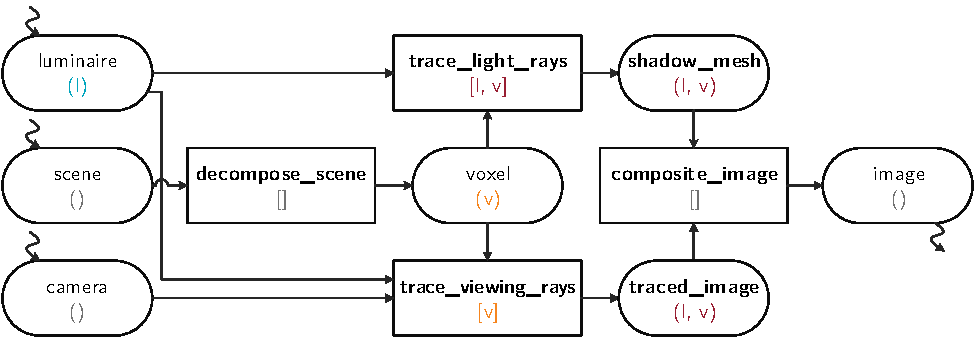
\includegraphics[width=\textwidth]{drawings/CnC.pdf}
  \caption{CnC Graph}
  \label{fig:cnc}
\end{figure}

Figure~\ref{fig:cnc} shows a graphical representation of the CnC graph, a 
textual version can be found in figure~\ref{fig:cnc-graph-text}.  Step 
collections  are represented as rectangles and data collections are represented
with ovals.  The tag collections for specific data or step collections are shown
in the shape.  The colors are used to group the similar tag collections. The 
control collection for the proposed model is static for all steps and is defined 
in an initialization step. The graph begins execution when the object, lights, 
and camera data are provided, and terminates when an image is produced.

\subsection{Tags}
The tags in CnC can be thought of as a way to index a specific step or data 
collection.  The elements in our tags are \textbf{frame}, \textbf{i}, 
\textbf{j}, and \textbf{k}.  The \textbf{frame} tag refers to one specific frame 
in the case of an animation or multiple views from different camera positions. 
The \textbf{i}, \textbf{j}, and \textbf{k} tags are iterators over 3D spatial 
data, selecting a specific voxel. 

\subsection{Data Collections}
\label{sec:datacollections}

The \textbf{object} data collection contains input data for the domain from the
environment. Currently, this data is extracted from WaveFront
``\texttt{.obj}'' files. The \textbf{decompose\_domain} step collection
partitions this data into voxels, producing the \textbf{voxel\_object} data
collection. Objects that span multiple voxels are duplicated. The
\textbf{lights} data collection contains data pertaining to light sources. The
\textbf{voxel\_light} data collection contains the same information as 
\textbf{lights} plus a traced light mesh for each wall of a voxel. The 
\textbf{camera} data collection contains the location and direction of the 
camera. The \textbf{ray} and \textbf{traced\_ray} data collections contain the 
primary rays. The \textbf{image} data collection contains the final image data.

\subsection{Step Collections}

As mentions in Section~\ref{sec:datacollections} the \textbf{decompose\_domain}
step takes the data to be traced as input and produces subsets of that
data based on voxel decomposition. As load balancing is not a concern,
a uniformly-gridded voxel decomposition is sufficient. The number of
voxels produced is set at runtime and should be more than the number
of nodes available.

In order to reduce the communication of secondary rays,
the \textbf{distribute\_lights} step is responsible for distributing light
information to each voxel. This guarantees each voxel will not need
to communicate with any other voxels. The light information
produced for each voxel contains the original light sources as well as
a light source mesh for each light and each wall of the voxel. The
mesh is produced by tracing rays from each light source to uniformly
spaced points along a voxel wall.  Where the rays intersect the wall light 
information is stored, producing the mesh. If the ray is blocked, the ray in 
the light mesh is tagged as in shadow, see figure ~\ref{fig:light2}.

\begin{figure}[!htb]
\centering
\begin{subfigure}{0.49\textwidth}
 \centering
  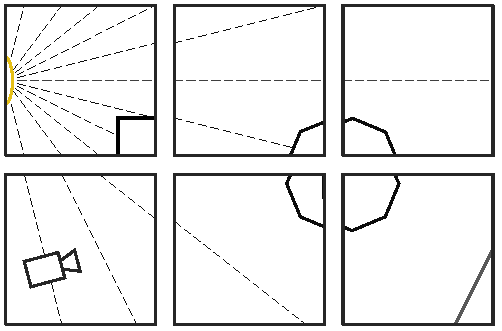
\includegraphics[width=.98\columnwidth]{drawings/Lights1.pdf}
  \caption{Initial light rays}
\end{subfigure}
\begin{subfigure}{0.49\textwidth}
 \centering
  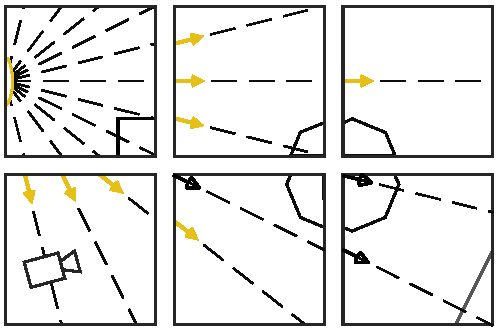
\includegraphics[width=.98\columnwidth]{drawings/Lights2.pdf}
  \caption{Computed light mesh}
\end{subfigure}
\caption{Light ray distribution}
\label{fig:light2}
\end{figure}

The \textbf{distribute\_rays} step is responsible for computing and distributing
the primary rays. 

\textbf{trace\_voxel} is the heart of the application. This step executes once 
for each voxel.  It traces the primary rays over its subset of the domain. If a 
ray intersects with an object the color is computed for the point. To determine 
illumination information, secondary rays from each light source are computed and 
the light mesh is used.  Rays that do not intersect objects within the voxels 
are left uncolored.  The step produces copies of the traced rays with the color 
either set or not if the ray intersected an object.

When all \textbf{trace\_voxel} steps have completed, the \textbf{produce\_image}
step merges the \textbf{traced\_rays} to compose the final image.  
Figure~\ref{fig:trace} a shows the primary rays as computed by the 
\textbf{distribute\_rays} step.  Figure~\ref{fig:trace} b shows the results of 
each voxel tracing the primary rays.  The rays that intersected each voxel are 
displayed and colored based on intersected objects.

\begin{figure}[!hb]
\centering
\begin{subfigure}{.49\columnwidth}
 \centering
  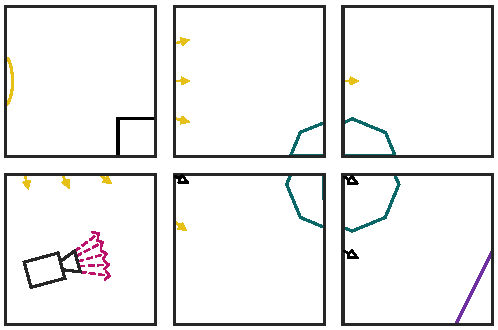
\includegraphics[width=.98\columnwidth]{drawings/Trace1.pdf}
  a) Distribute rays
\end{subfigure}
\begin{subfigure}{.49\columnwidth}
 \centering
  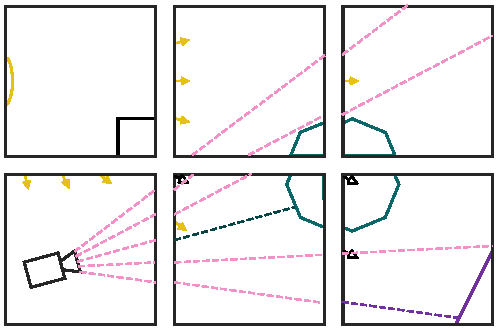
\includegraphics[width=.98\columnwidth]{drawings/Trace2.pdf}
  b) Trace voxel
\end{subfigure}
\caption{Ray tracing example}
\label{fig:trace}
\end{figure}

\newpage

\section{Algorithm}
The implemented ray tracer can be broken down into the five step collections
outlined in the CnC graph file.  Pseudo code for each step is presented in this
section.  We walk through an example use case in chapter~\ref{sec:evaluation}.

\subsection{Decompose domain}
Decompose domain reads and splits a .obj file into voxel subsets.  The amount of
voxels the domain is divided into is up to the user at runtime.  Pseudo code can
be found in figure~\ref{fig:decompose-domain}.  

\begin{figure}[!htb]
\begin{algorithm}
DECOMPOSE_DOMAIN(scene, v)
  in:  the scene to be traced
       number of voxels, v
  out: v subsets of data
  voxels[v]
  for all voxel in voxels do
    for all trangles in scene do
      if trangle is in voxel then
        voxel.data.add(trangle)
      end if
    end for
  end for
return voxels
\end{algorithm}
\caption{Decompose domain pseudo code}
\label{fig:decompose-domain}
\end{figure}

The code implemented supports quad and triangle geometry as well as materials.  
As Embree does not support textures, any material using a texture is modified to
use a solid color.  A triangle or quad is considered in a voxel if any of its
vertices are in the voxel.  This results in geometry that crosses voxel walls 
being duplicated in neighboring voxels. 

\subsection{Distribute lights}
\label{sec:distribute-lights}
Distribute lights generates light meshes for each light source.  The light 
meshes can be thought of as a mesh of vertices on each voxel wall.  Each vertex
in the mesh contains light information that can be used by the voxel computation
to illuminate any point the viewing rays intersect.  Pseudo code for the 
algorithm can be found in figure~\ref{fig:distribute-lights}. 

\begin{figure}[!htb]
\begin{algorithm}
DISTRIBUTE_LIGHTS(lights, voxels) 
  in:  lights in the scene
       voxel data
  out: light mesh for each voxel
  for all light in lights do
    light_mesh = false;
    for all voxel in voxels do 
      if not light_mesh then
        light_mesh = 
          COMPUTE_MESH(light, voxel)
      else
        light_mesh = 
          PROPIGATE_MESH(light_mesh, 
                       light, voxel)
      end if
      light_mesh_ = COPY(light_mesh)
      voxel.light_meshes.add(light_mesh_)
    end for
  end for
return voxels
\end{algorithm}
\caption{Distribute lights pseudo code}
\label{fig:distribute-lights}
\end{figure}

For each light in the scene, distribute lights creates light ray samples from
the light and distributes them into the domain.  Currently the algorithm 
supports directional and point light sources, but could be extended to support 
other types.  Each ray sample generated is cast into the scene starting with the
closest voxel and propagating outward.  The density of the samples is set by the
user at runtime.  If the rays intersect an object within a voxel the ray is 
marked as in shadow before being propagated to the next voxel.  This results in 
a mesh of rays, originating on each voxel wall marked as either in or not in
shadow.  The mesh also contains information about which light source it was 
generated from.  

\subsection{Distribute rays}
Distribute rays is responsible for computing all the primary rays from a camera
position.  The distribution of the primary rays is handled by the Embree core
ray tracing library and is not presented here.

\subsection{Trace voxel}
label{sec:trace-voxel}
Trace voxel uses the voxel data set, the light meshes, and the primary rays to 
trace its subset of the scene.  This method produces a traced copy of the 
primary rays with color information on the rays that intersect objects within 
the voxels subset of the domain.  Pseudo code can be found in 
figure~\ref{fig:trace-voxel}.

\begin{figure}[!htb]
\begin{algorithm}
TRACE_VOXEL(rays)
  in: all primary rays
  out: all primary rays with color computed
  for all ray in rays do
    if ray intersects scene then
      for all light in lights do
        light_ray <- RAY(ray, light)
        if not light_ray intersects scene
          if voxel.light_meshes[light].
            CLOSEST(light_ray).IS_IN_SHADOW
              ray.color += COMPUTE_COLOR(ray, light)  
          end if           
        end if      
      end for
    else
      ray.color <- FALSE
    end if
  end for
return rays
\end{algorithm}
\caption{Trace voxel pseudo code}
\label{fig:trace-voxel}
\end{figure}

The Embree library is used to determine if the primary rays intersect the scene.
Only rays that intersect the scene are colored.  The algorithm to determine the
color at an intersection point is close to that of a typical ray tracer, but has
been modified to use the light mesh to determine if light rays intersected an 
object outside the current voxels subset of data.  

A typical ray tracer calculates a light ray from each intersection point to each 
light source.  The light rays are then cast into the scene towards the light, if
they intersect an object, the ray is considered as in shadow and no light 
contribution is considered to illuminate the intersection point.  Our algorithm
has pre-calculated a sampling of the light rays in the light mesh and can use 
this information to replace casting the lights into the entire domain.

For each intersection point, light rays are calculated towards each light 
source.  The light ray is cast into the current voxel, if the ray is blocked by
an object within the current voxels data, we know the ray is in shadow and the
light mesh is not needed.  If the ray reaches a voxel wall, the light mesh must
be used to determine if the ray is in shadow or not.  We use a nearest neighbor 
approach to find the closest vertex on the mesh wall to the intersection point 
of the light ray and the wall.  If that vertex has been marked as in shadow, we
consider the light ray as in shadow.  If not, the light is used to illuminate 
the primary rays intersection point.  This is illustrated in 
figure~\ref{fig:light-mesh-intersection}.  

\begin{figure}[t]
  \centering
  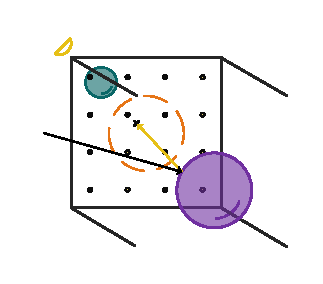
\includegraphics[width=8cm]{drawings/LightIntersection.pdf}
  \caption{Light mesh intersection}
  \label{fig:light-mesh-intersection}
\end{figure}

Figure~\ref{fig:light-mesh-intersection} shows a viewing ray entering a and
intersecting a purple sphere.  The light ray from the intersection point to the 
light source is computed and traced to the voxel wall.  No objects obstruct the
light ray within the voxel so the light mesh is used to determine if the 
intersection point is in shadow.  The closest vertices to the light mesh have 
been highlighted with an orange circle.  The vertex closest to the light ray and 
voxel wall intersection is the upper right hand corner of the highlighted 
vertices and is in shadow having been blocked by the blue sphere.

\subsection{Compose image}
The final method in our algorithm, compose image, takes the results of each
call to trace voxel and produces the final image.  Pseudo code can be found in
figure~\ref{fig:compose-image}.  

\begin{figure}[!htb]
\begin{algorithm}
COMPOSE_IMAGE(traced_rays[])
  in: traced rays from each voxel,
      sorted back to front
  out: image, a ray traced scene
  for all rays in traced_rays do
    for all ray in rays do
      if(ray.color) then
        image[ray.orgin.x][ray.orgin.y].color = ray.color;
      end if
    end for
  end for
return image
\end{algorithm}
\caption{Trace voxel pseudo code}
\label{fig:compose-image}
\end{figure}

Each ray traced may have intersected an object in multiple voxels.  Since the 
trace computations are independent and do not communicate, it is up to compose
image to ensure the final image uses the intersection point closest to the 
viewer.  We do this by tracing the rays starting with the voxel farthest from
the view point and working backwards towards the viewer.  For each set of traced
rays we iterate over the rays.  If the ray has been colored, we color the pixel
the ray represents.  As we iterate closer to the viewpoint, pixel colors are
overridden by closer intersections, producing a correct final image. 


















